% !TEX root = ../PhD Thesis.tex
\chapter{cTRAP: identification of candidate causal perturbations from differential gene expression data}
\label{chap:ctrap}

During a lab retreat to Madeira in 2017, we focused our attention to what were the objectives of the lab and what we can provide to the community. One of the ideas seemed easy to do: comparing a custom differential gene expression against a large database of differential expression profiles.

The idea was already been hinted in the original paper of CMap and usable through their online tool at \url{https://clue.io}, but there were issues with their implementation.

The Connectivity Map or CMap (Subramanian et al., 2017) is a repository of transcriptomic signatures for thousands of genetic (gene overexpression or knockout) and pharmacological perturbations tested in human cancer cell lines. We developed cTRAP (\url{https://bioconductor.org/packages/cTRAP}), an R/Bioconductor package to compare user-provided differential gene expression profiles with those from CMap, allowing to infer putative candidate molecular causes for the observed differences, as well as compounds that may promote or revert them. The comparisons are made based on correlation and gene set enrichment (Subramanian et al., 2005) approaches.

The most recent feature of cTRAP is its visual interface, allowing users to interactively explore their results. The associated manuscript (of which I am a co-first and co-corresponding author) is in preparation for submission to an international peer-reviewed scientific journal.

-- Functions to deal with dummy/mock object

\section{Benchmarking + code/memory optimisation}

\section{Graphical interface}

cTRAP has one modular interface that allows to 

This was an experiment that combines using explicit R commands via an helpful graphical interface.

\subsection{Web server support}
\label{sec:ctrap-web}

In order to increase its usefulness to the scientific community, we made cTRAP available online\footnote{More information in \fullref{chap:app-server}} with a single interface to perform all the analyses and plots in cTRAP. A clear question arrived with such strategy: how to deal with long-running tasks? The way R/Shiny is built, an entire cTRAP section would be kept online and consuming useful resources, but this would not properly scale for multiple users using heavy memory simultaneously, for instance. To avoid this, long-running tasks are performed in the background. But this also meant that the users would need get their results back afterwards. And thus the idea of sessions was born.

In practical terms, cTRAP sessions are folders that are created in a directory based on a random, unique string of numbers and letters, henceforth denominated as a \emph{token}. Each folder holds all the data for a session and either the associated token can be kept or the session data can be downloaded as a single RDS file. All data changes performed in the scope of the current session are saved into the respective folder.

When going to cTRAP in the next visit, the user is greeted with a welcome screen that allows to create a new session or load a previous one by either giving a token or a RDS file. The RDS file has another advantage: it ensures the user can open the data in an R session in their local computer given that this RDS file is simply a list of all the datasets available in the session or even use this file in a local version of cTRAP. Moreover, as sessions start to accumulate in our server, they may be removed from the system and thus may be inaccessible.

\begin{figure}[!ht]
  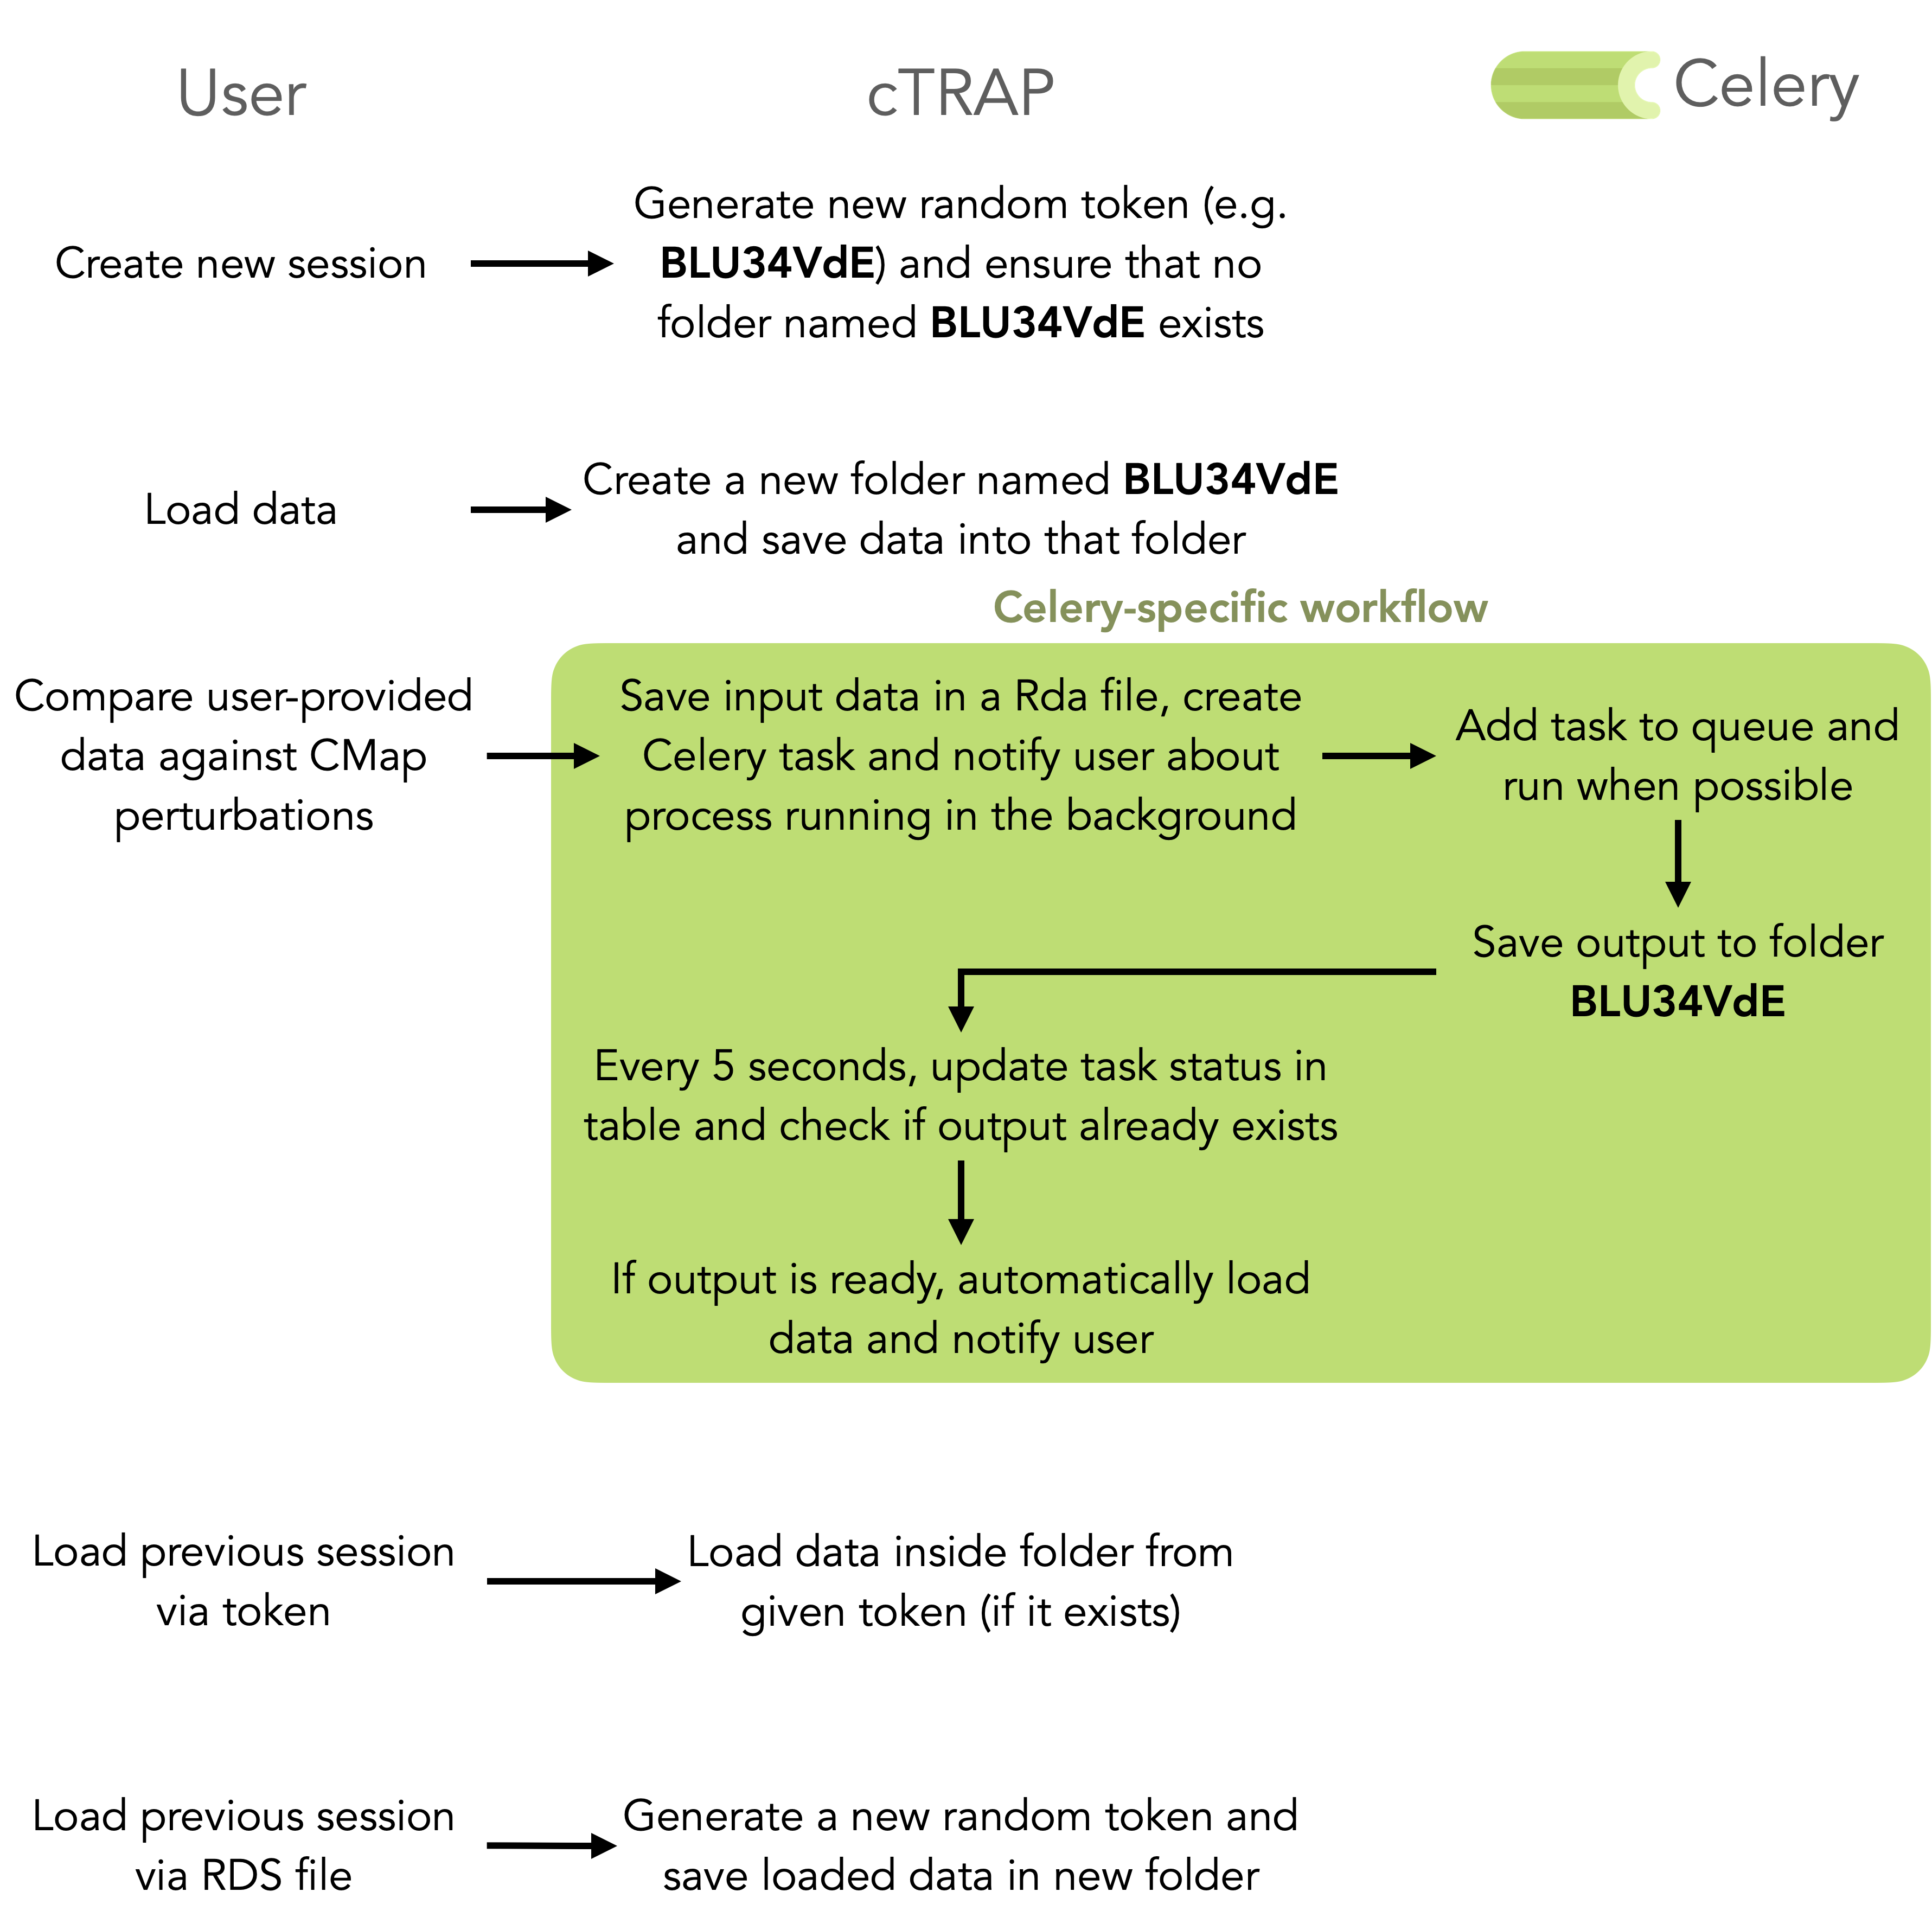
\includegraphics[width=0.8\textwidth]{images/ctrap/celery}
  \centering
  \caption{Interaction between the user, cTRAP and Celery.}
\end{figure}

To run tasks in the background, I decided to use Celery, a task queue manager written in Python, and Flower, a Celery monitoring app that also provides a useful RESTful API to work with Celery. Flower makes it easier to send tasks to Celery via HTTP methods, facilitating the communication between cTRAP and Celery. To make use of Flower in R, I created floweRy, an R package to help create the commands used in the Flower API more easily.

However, cTRAP can also run the session feature without Celery/Flower support. It works similarly, but the tasks are run in the same R process (as usual in an R/Shiny app) so the user has to wait for the long-running tasks to finish before proceeding with interacting with the app. Another limitation is that if cTRAP times out or is shut down, the running processes will stop.

Most data used for the analyses in cTRAP are the same across sessions with the exception of the differential expression data. In the implementation of our app server, the common cTRAP data is available in a folder accessible to all sessions, thus skipping the step of downloading and preparing the data.

During the whole process, the user interface shows tables with the status of each job from the user. When the process finishes running, the data is automatically loaded and a notification in cTRAP alerts the user that the data is now loaded and ready to visualise.
